\documentclass{article}

% Packages for various functionalities
\usepackage[utf8]{inputenc} % Encoding of the document
\usepackage[T1]{fontenc} % Font encoding
\usepackage{amsmath,amssymb} % Mathematical symbols and environments
\usepackage{graphicx} % For including images
\usepackage{cite} % For managing citations
\usepackage{caption} % Customizing captions
\usepackage{lineno} % Line numbers
\usepackage{lipsum} % For generating dummy text (remove this line)
\usepackage{booktabs} % For professional-looking tables
\usepackage{xcolor}



% Title and authors
\title{Comparative Study of Neural and Classical Retrieval Methods for FANDOM Wikis}
\author{Author1\thanks{Corresponding author: email@example.com} \and Author2 \and Author3}
\date{\today}

\begin{document}

\maketitle

\begin{abstract}
This is the abstract of your paper.
\end{abstract}

\section{Introduction}
% Your introduction here

\section{Datasets}
% Your introduction here

\section{Retrieval Methods}
\subsection{Classical Retrieval Methods}
% We employed the TF-IDF method for classical retrieval. TF-IDF calculates the importance of a term in a document by considering its frequency in the document and its inverse frequency in the entire corpus.

\subsection{Neural Retrieval Methods}
For our neural retrieval approach, we adopted the ColBERT \cite{khattab2020colbert} model , which utilizes Transformer models to generate vector embeddings for word tokens in a text sequence. These embeddings capture the contextual information of the tokens within the sequence and are then used to calculate the similarity between two sequences.

\subsubsection{ColBERT Model}
The ColBERT model takes a query and a document passage as input. These strings are then tokenized using a Transformer model's associated tokenizer, resulting in sequences of query tokens ($q = q_0q_1\dots q_m$) and document tokens ($d = d_0d_1\dots d_n$). Next we prepend a \texttt{[CLS]} token at the beginning and append a \texttt{[SEP]} token at the end of both sequences and add either a \texttt{[Q]} or \texttt{[D]} token after the \texttt{[CLS]} token to encode the input sequence type (query or document/passage). The query and document sequences are constrained to maximum lengths of $N_q$ and $N_d$ tokens, respectively. If the query is shorter than $N_q$ tokens, we pad the sequence with \texttt{[MASK]} tokens until it reaches length $N_q$. The document sequence will not be padded if shorter than $N_d$ and will be of length $L_d = min(n + 3, N_d)$. Thus, the input sequences for the ColBERT model are as follows: $q = \texttt{[CLS]}\texttt{[Q]}q_0q_1 \dots q_m\texttt{[SEP]}\texttt{[MASK]}\dots\texttt{[MASK]}$ and $d = \texttt{[CLS]}\texttt{[D]}d_0d_1 \dots d_{n}\texttt{[SEP]}$, respectively. These tokenized sequences are then passed through a Transformer model's Encoder, with experiments conducted using both BERT \cite{devlin2019bert} and RoBERTa \cite{liu2019roberta} architectures. The resulting output is a sequence $E = E_1E_2 \dots E_k$ of high-dimensional vectors, where $k$ corresponds to $N_q$ or $L_d$, depending on the sequence being processed. These vectors are subsequently mapped to a lower dimensionality $d$ using a linear transformation. To calculate the similarity between the query and document sequences, we employ the "sum of maximum similarity" method, as presented in the ColBERT paper. However, instead of using the sum, we use the mean to obtain the similarity score. The function is computed as follows:
$$ S(q,d) := \frac{1}{N_q} \sum_{i=1}^{N_q} \max_{j = 1, \dots, L_d} sim(E_{q_i}, E_{d_j})
$$
We evaluate similarity using both cosine similarity and negated squared $L_2$-norm. The formulas for the similarity measures are as follows:
$$
sim_{cos}(E_{q_i}, E_{d_j}) := \frac{1}{\| E_{q_i} \|\| E_{d_j} \|} E_{q_i}^TE_{q_j} 
$$

$$
sim_{L2}(E_{q_i}, E_{d_j}) := -{\| E_{q_i} -E_{d_j} \|}^2
$$

$$
sim_{L2,norm}(E_{q_i}, E_{d_j}) := -{\| \frac{E_{q_i}}{\| E_{q_i} \|}  - \frac{E_{d_j}}{\| E_{d_j} \|} \|}^2
$$
In the ColBERT paper, the vectors were normalized before applying these similarity measures. However, we also experimented with $L_2$-norm without normalization of the embedding vectors.

\subsubsection{ColBERT Training}
During the training the BERT/RoBERTa encoder is fine-tuned and the last linear projection and the additional \texttt{[Q]}/\texttt{[D]} tokens are learned from scratch. For training on the MS MARCO \cite{bajaj2018ms} dataset, the model receives batches of tuples in the form $\langle q_i^+, d_i^+, d_{i, 1}^-, \dots, d_{i, 9}^-\rangle$. Here, $d_i^+$ represents the answer passage for the query $q_i^+$, and the passages $d_{i, l}^-$ do not contain the answer. When training on our FANDOM QA dataset, the model receives batches of tuples in the form $\langle q_i^+, q_i^-, d_i^+\rangle$, where $q_i^+$ is answered by $d_i^+$ while $q_i^-$ is not. Despite the differences in data format, the training objective remains the same: maximizing the similarity between the answering query/passage pairs relative to the other given passages. The loss is calculated using the cross-entropy loss and is defined as follows for the MS MARCO dataset:
$$
\ell = -\frac{1}{B} \sum_{i=1}^{B} \log \frac{e^{N_q S(q_i^+, d_i^+)}}{e^{N_q S(q_i^+, d_i^+)} + \sum_{j=1}^{9}{e^{N_q S(q_i^+, d_{i, j}^-)}}}
$$
For the FANDOM QA dataset, the loss function becomes:
$$
\ell_i = -\frac{1}{B} \sum_{i=1}^{B} \log \frac{e^{N_q S(q_i^+, d_i^+)}}{e^{N_q S(q_i^+, d_i^+)} + e^{N_q S(q_i^-, d_i^+)}}
$$
Sadly, it is necessary to manually scale the similarity scores by a factor of $N_q$ in order to achieve better convergence during training (so we actually use the sum of maximum similarity for training). The reason behind this requirement is likely attributed to the range of cosine similarity scores, which typically fall between -1 and 1. Even in an ideal scenario where predicted similarities take the form of $\langle 1, -1, \dots, -1\rangle$, applying the softmax function yields probabilities such as $\langle 0.451, 0.061, \dots, 0.061\rangle$, which is similar to using extremly aggressive label smoothing \cite{szegedy2015rethinking}. Unfortunately, we have not been successful in devising an alternative loss function to address this limitation.

We also conducted experiments using Mean Squared Error (MSE) loss in combination with cosine similarity. In this setup, the target for the loss function was set to 1 for the pairs $\langle q, d^+\rangle$ representing answering passages. Conversely, for the pairs $\langle q, d^-\rangle$ representing not answering passages, we enforced orthogonality by aiming for a cosine similarity of 0. However, this approach yielded inferior performance, as demonstrated in the subsequent analysis.


\subsubsection{Retrieval with ColBERT}
Due to the computational cost associated with calculating the similarity between a given query and all passages, we adopt the two greedy methods from the original ColBERT paper: "reranking" and "full-retrieval." In the "reranking" approach, we employ a classical retrieval algorithm (in our case, TF-IDF) to retrieve the top-$k$ passages for a query. Subsequently, ColBERT is used to re-rank these $k$ documents based on their similarity scores. On the other hand, "full-retrieval" exclusively utilizes ColBERT. For a given query, we search for the top-$\hat{k}$ most similar document embedding vectors for each of the $N_q$ query embedding vectors. We retrieve the associated documents ($\leq \hat{k}N_q$ unique documents) and calculate the similarity between the query and these documents. Finally, we return the top-$k$ documents. Similar to the original paper, we set $\hat{k} = k / 2$, although values like $\hat{k} = k / 5$ seem to yield similar performance while reducing the number of passages to rank and thus saving inference time.

\section{Results}
% Your results here


Example table:
\begin{table}[htbp]
    \centering
    \label{tab:hyperparameters}
    \begin{tabular}{ccccccc}
      \toprule
      \textbf{Method} & \textbf{MRR@10}  & \textbf{RECALL@1} & \textbf{RECALL@10} & \textbf{RECALL@50} \\
      \midrule
      TF-IDF & Value 1.1 & Value 1.2 & Result 1  & Result 1 \\
      $\text{ColBERT}_\text{rerank}$ & Value 2.1 & Value 2.2 & Result 2 & Result 1 \\
      $\text{ColBERT}_\text{full}$ & Value 3.1 & Value 3.2 & Result 3 & Result 1 \\
      % Add more rows as needed
      \bottomrule
    \end{tabular}
    \caption{Hyperparameters and Results}
\end{table}

\section{Interpretability}
% Your discussion here

\section{Model Understanding}
As part of our research, we aimed to understand how COLBERT works and identify its strengths and weaknesses.
To accomplish this, we visualized the tokens in the passage that hold high relevance for COLBERT. One of the objectives
was to locate the answer to the question within the passage and present it to the user.
ColBERT utilizes the similarity between query vectors and passage vectors to determine the correct passage.
Our research has confirmed a strong relationship between query tokens $q_i$ and query vector $E_{q_i}$, as well as between
passage tokens $d_j$ and passage vector $E_{d_j}$.
Therefore, a passage token $d_j$ is considered relevant to ColBERT regarding
a question q if the associated vector $E_{d_j}$ contributes to a high similarity score $S(q, d)$.
This occurs when $E_{d_j}$ exhibits a high similarity to one or multiple query vectors $E_{q_i}$.
The relevance of a passage vector $d_j$ can be determined by the number of query vectors that exhibit high similarity
to $E_{d_j}$.
$$
    R_{absolute}(q, d_l) = \:\mid \{E_{q_i} \mid E_{d_l} \in \underset{j = 1, \dots, N_d}{max_k} sim(E_{q_i}, E_{d_j})\} \mid,
$$
where $max_k(U) = \{a_1, a_2, \dots, a_n\}$ such that $a_1 = max(U), a_2 = max(U \setminus \{a_1\}), \dots, a_n = max(U \setminus \{a_1, a_2, \dots, a_{n-1}\})$.
In our study, we identified the two most ($k=2$) relevant passage vectors for each query vector.
We choose k=2 to strike a balance between marking a sufficient amount of information without assigning high relevance to every passage token. 
Considering that the queries are encoded into $32$-dimensional vectors, 
this yields a total of $k*32=64$ one-dimensional data points, which range from $0$ to $N_d$ and represent one passage token each.
Therefore, the relevance function $R_{absolute}$ can be viewed as a histogram that represents the distribution of these $64$ data points.

It is evident that the relevance of a passage vector depends not only on its frequency among the top k similarities of the query vectors
 but also on the value of each individual similarity.
In light of this, we have expanded the similarity score $R_{absolute}$ to the metric $R_{added\_values}$:
$$
	R_{added\_values}(q, d_l) = \sum_{E_{q_i} \in D} sim(E_{q_i}, E_{d_l}) \text{, with } D= \{E_{q_i} \mid E_{d_l} \in \underset{j = 1, \dots, N_d}{max_k} sim(E_{q_i}, E_{d_j})\}.
$$

Given our objective of not only highlighting individual tokens in the passage as particularly relevant but also identifying the range likely to contain the answer to the question, we utilize Kernel Density Estimation (KDE)\cite{kde} as an additional approach. 
KDE is a statistical method used to estimate the probability density function to a given data sample, enabling us to identify a range of passage tokens
that holds significant priority for COLBERT.
In other words, when multiple tokens within a specific range exhibit high relevance scores and are densely clustered together, it signifies the importance of that particular range in the broader context.
Simplified, Kernel Density Estimation (KDE) generates a density function by overlaying kernels, such as normal distributions.
In this process, each data point contributes a kernel that is shifted based on the position of the data point.
One of the benefits of using KDE is that it provides a smooth and continuous estimation of the probability distribution. 
Additionally, KDE does not require the specification of additional parameters beyond the choice of kernel and bandwidth, 
which determines the level of smoothing.

\begin{figure}[h]
	\centering
	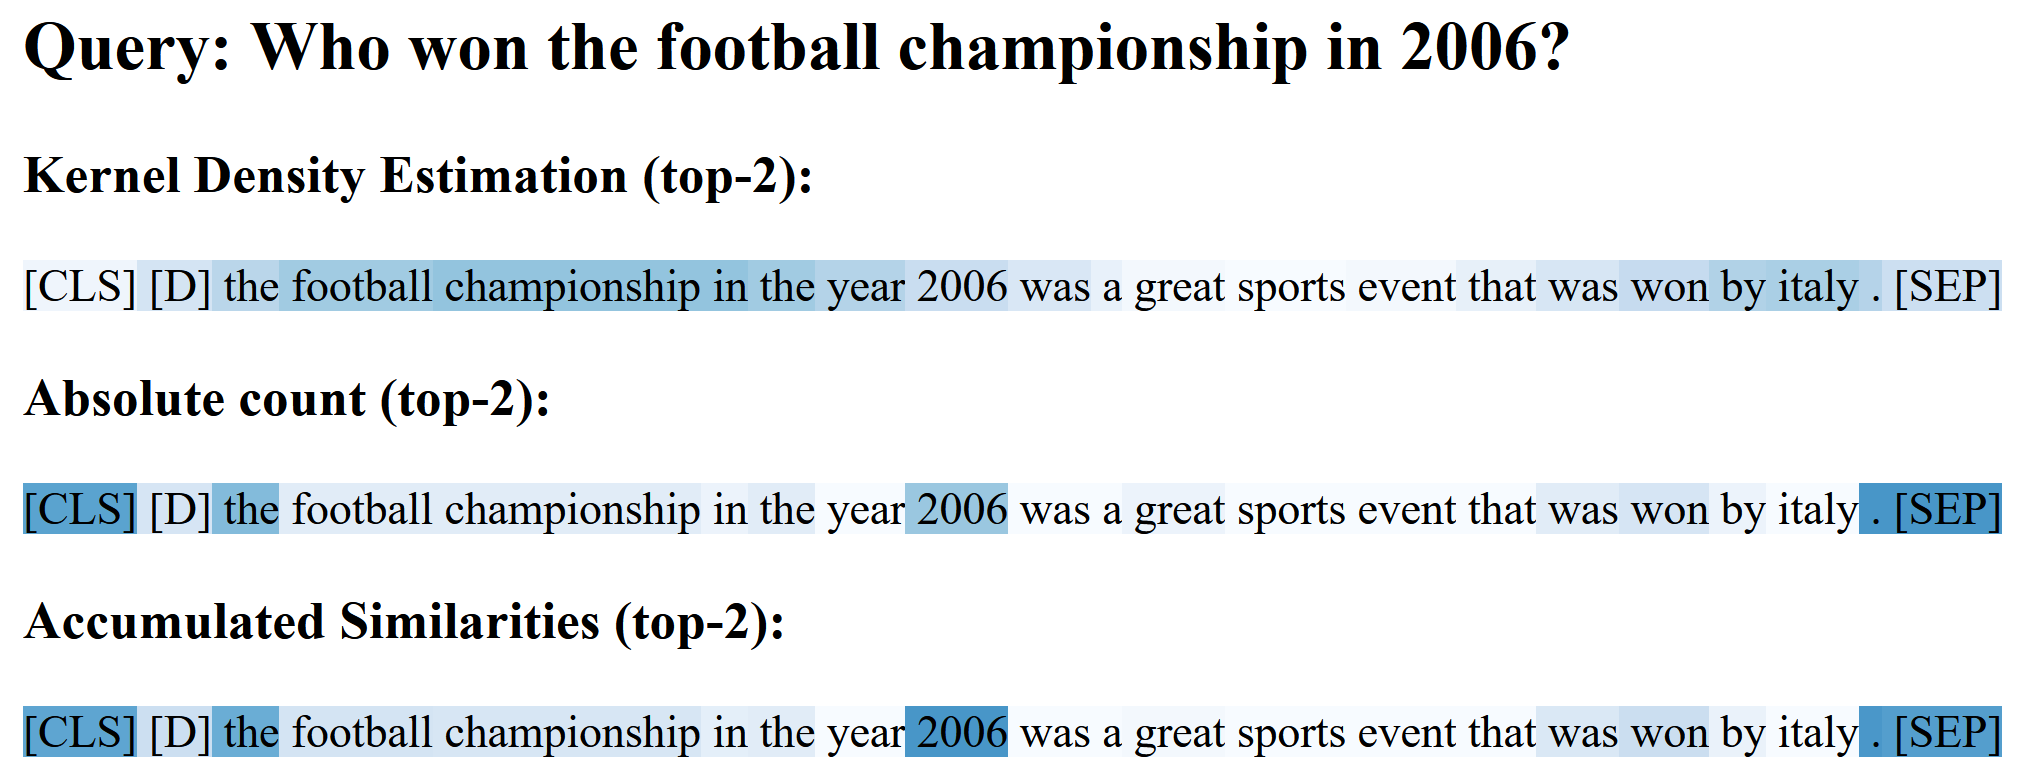
\includegraphics[width = 13cm]{"../ressources/results/football_html.png"}
	\caption{example1}
	\label{fig:example1}
\end{figure}

ColBERT reliably identifies the passage containing the answer to the given question by comparing the passage embedding with the query embedding. 
However, in most cases, the answer cannot be directly identified by comparing the embedding of the passage with the embedding of the query.
In most instances, the words in the passage that exhibit the highest similarity with the query are not the answer itself, but rather the words 
that lead to the answer.
When comparing the query "Who won the football championship in 2006?" and the passage "The football championship in the year 2006 was a great 
sports event that was won by Italy."~\ref{example1} the highest similarity will be found in the words "the", "championship", "2006", "was", 
"won" and "by" instead  of the actual answer "Italy", because the actual answer is not relevant to decide whether the question is answered 
in the passage. 
Colbert was not trained to find the answer, but rather to determine whether the answer is contained within the passage.
Substituting any other word for "Italy" would have minimal impact on the probability of the passage providing an answer to the question.
Kernel Density Estimation (KDE) partially addresses this problem by assuming that the answer is likely to be located in the areas of the passage 
that contain a higher concentration of relevant tokens with respect to the question.
The tokens \texttt{[CLS]}, \texttt{[D]} and \texttt{[SEP]} are ignored by KDE.
The markings aid the user in swiftly identifying the likely location of the answer within the passage. Moreover, the markings elucidate the 
significance of the retrieved passage to Colbert. 
In the event that the answer is not present in the passage, the user can hopefully discern the reasons for Colbert's failure and
subsequently modify the query accordingly.
 
\begin{figure}[h]
	\centering
	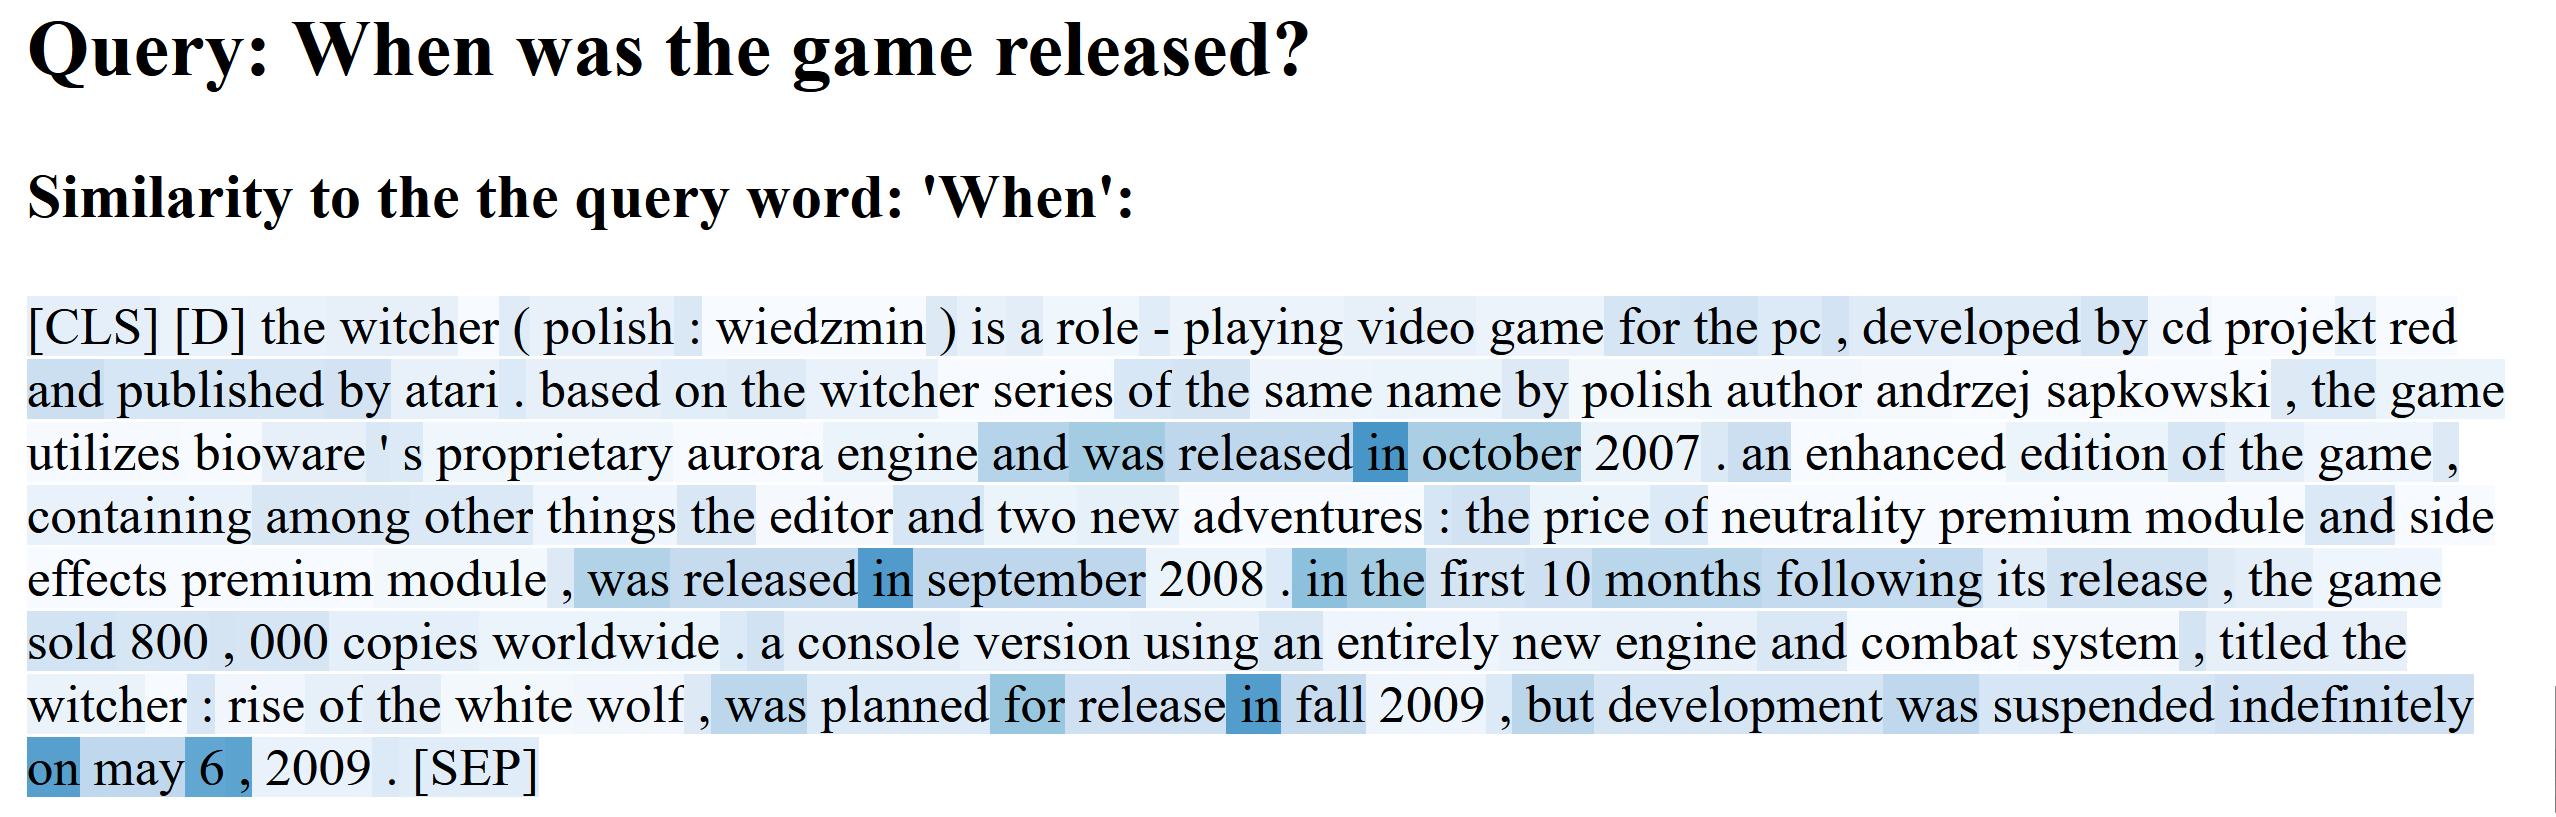
\includegraphics[width = 13cm]{"../ressources/results/when_html.png"}
	\caption{example2}
	\label{fig:example2}
\end{figure} 
 
 The major strength of Colbert lies in its understanding of semantics, where words are not considered in isolation but in context. However, Colbert encounters similar issues as single-word-based systems like TF-IDF. In Example 2, the similarity for the word 'when' is visualized. Evidently, Colbert comprehends the intended meaning behind the interrogative word 'when.' Nevertheless, Colbert often misses the mark in answering the question and instead retrieves passages that provide extensive information about the content of the question. Colbert is easily distracted by passages that extensively cover the topic of the question. Passages that succinctly provide the answer but have a different core topic are overlooked by Colbert. Additionally, it seems that insufficient attention is given to the interrogative word.
 This behavior can be explained by the fact that during the training phase, there are only a few passages that contain substantial information about the topic of the question but do not directly answer the question.
 
%
%Absolute count: This mode considers only the number of queries per passage.
%
%Added values: This mode sums the similarities between the query vectors and the passage vectors.
%
%Kernel Density Estimation (KDE): KDE is a statistical method used to estimate the probability distribution. It is employed to identify not only individual important tokens but also a range that has high priority for COLBERT. By using a Gaussian kernel (density function), KDE attempts to represent a sample as an overlay of scaled and shifted kernels. In simple terms, it assumes a normal distribution for each "value" and sums them up. The output of KDE is a probability distribution, where a higher density of points in a specific range indicates a higher likelihood of their occurrence.
%
%"Kernel density estimation is a technique for estimating the probability density function, which is essential for enabling the user to analyze the studied probability distribution more effectively compared to using a traditional histogram. Unlike the histogram, the kernel technique provides a smooth estimate of the PDF, utilizes the locations of all sample points, and more convincingly suggests multimodality."
%

\section{Conclusion}
% Your conclusion here



% Uncomment the following lines for including references
\bibliographystyle{plain}
\bibliography{references}



\end{document}
